\documentclass[11pt]{article}

\usepackage[margin=1in]{geometry}
\usepackage{graphicx}
\usepackage{booktabs}
\usepackage{amsmath,amssymb}
\usepackage{microtype}
\usepackage[colorlinks,citecolor=blue,urlcolor=blue,linkcolor=blue]{hyperref}
\usepackage{xcolor}
\usepackage{enumitem}
\usepackage{caption}

\setlength{\parskip}{0.5em}
\setlength{\parindent}{0em}

\title{Experiment~4: IQL vs.\ OA-IQL vs.\ MAPPO\\on the Resource-Augmented Predator-Prey Task}
\author{Rajdeep Singh \\ REL Lab, USC}
\date{May 2026}

\begin{document}
\maketitle

%% ------------------------------------------------------------------
\section{Summary}

We train three multi-agent RL algorithms---Independent Q-Learning
(IQL), Opponent-Aware IQL (OA-IQL), and Multi-Agent PPO
(MAPPO)---on a \textbf{resource-augmented predator-prey task} designed
to produce qualitatively distinct prey strategies.  All runs use 2\,M
environment timesteps, 3 seeds, random (mixed circle/corners) resource
placement.

\textbf{Main finding.}  MAPPO predator returns are roughly $3\times$
higher than either IQL variant (+110.5 vs.\ +33--36), confirming
that IQL is underperforming on this task.  The gap is attributable to
MAPPO's centralized critic, which sees all agents' observations during
training and can coordinate predator movements.  OA-IQL edges IQL on
predator return (+35.5 vs.\ +33.5) but the difference is within noise
at 3 seeds.  Resource collection rates are comparable across all three
algorithms ($\sim$0.4--0.5 per step), so the return gap is driven
entirely by the tag/evasion component.


%% ------------------------------------------------------------------
\section{Task design}

\texttt{SimpleTagResourcesMPE} extends the base simple-tag
environment with 4 collectable resource tokens:

\begin{itemize}[nosep]
  \item \textbf{Only the prey} sees resource positions (obs:
        14-d base $+$ 12-d resource $=$ 26-d).
  \item \textbf{Only the prey} can collect them (approach within
        $r=0.15$), earning $+5.0$ reward each.
  \item Predator observation is unchanged (16-d).
\end{itemize}

Three placement modes: \emph{circle} (radius 0.6), \emph{corners}
($\pm 0.8$), and \emph{random} (50/50 mixture).  The random mode
produces a bimodal trajectory distribution by construction.


%% ------------------------------------------------------------------
\section{Algorithms}

\begin{description}[style=nextline,font=\normalfont\bfseries]
\item[IQL] Independent Q-Learning.  128-dim MLP, replay buffer
  (size 5000, batch 32), $\epsilon$-greedy ($1.0 \to 0.05$,
  10\% decay), $\gamma{=}0.9$, LR\,$=$\,0.005.
  (\texttt{iql\_teams\_mlp.py})

\item[OA-IQL] Same trunk, adds an opponent-action prediction head
  (cross-entropy loss, coef\,$=$\,0.5).  At eval, the opp head is
  used for MC planning ($K{=}5$ rollouts, $H{=}3$ horizon).
  (\texttt{iql\_teams\_oa\_mlp.py})

\item[MAPPO] Per-team actor + centralized critic (concatenated obs).
  PPO clipped surrogate, GAE ($\lambda{=}0.95$), $\gamma{=}0.99$,
  32 envs $\times$ 128 steps, 4 PPO epochs per update.
  (\texttt{mappo\_teams\_mlp.py})
\end{description}


%% ------------------------------------------------------------------
\section{Results}

\subsection{Training curves}

Figure~\ref{fig:curves} shows learning dynamics over 2\,M timesteps.
IQL/OA-IQL curves are \emph{greedy test returns} (evaluated every
5\% of training); MAPPO curves are on-policy training returns.  The
x-axis is environment timesteps so the algorithms are directly
comparable despite different batch sizes.

\begin{figure}[h]
  \centering
  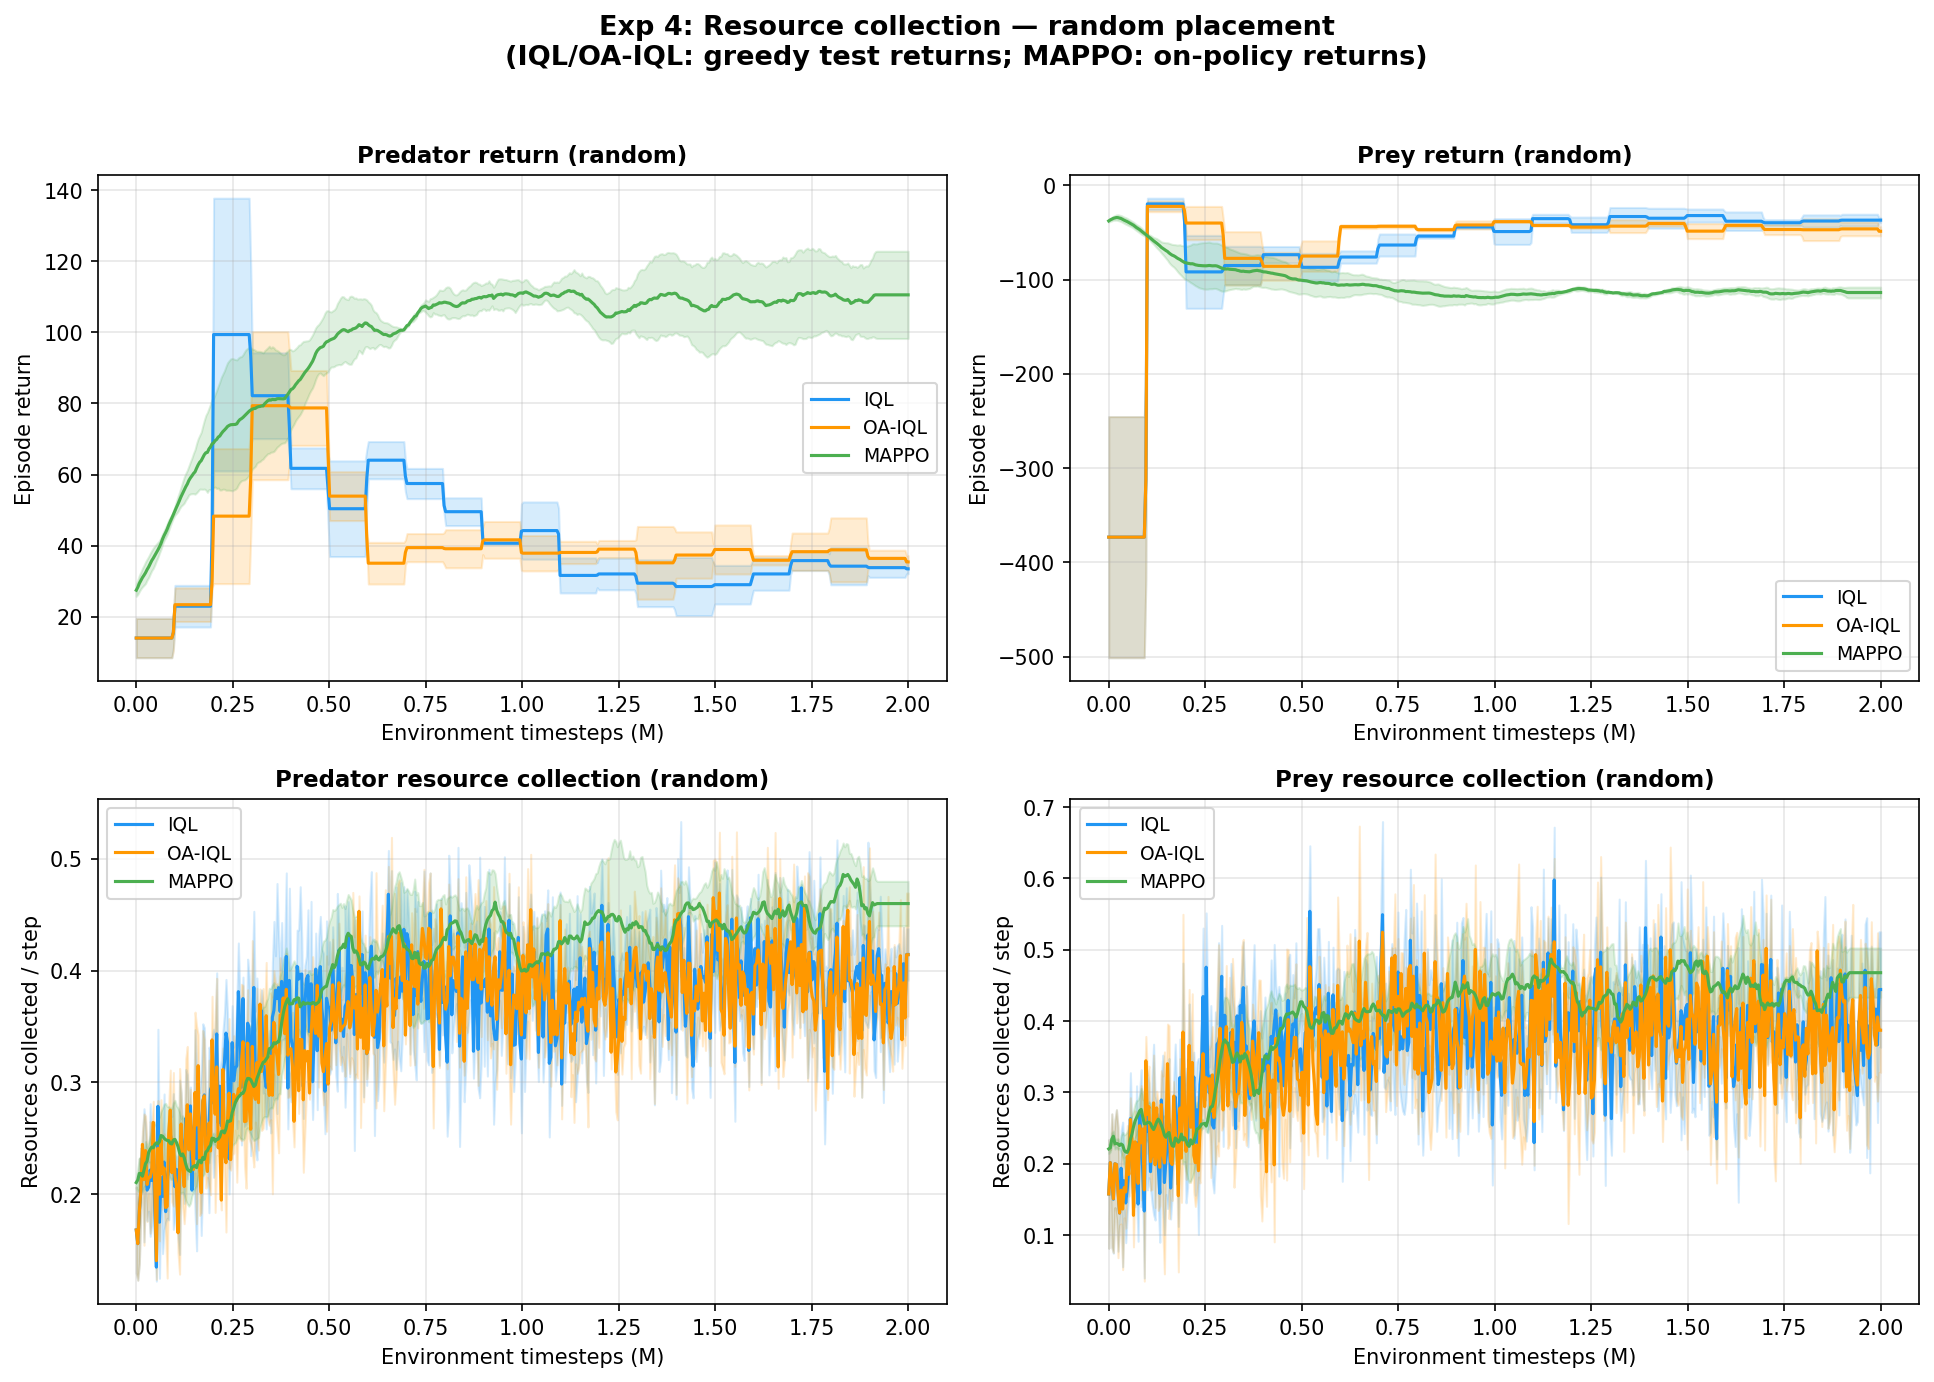
\includegraphics[width=\textwidth]{../plots/exp4_training_random.png}
  \caption{Exp~4 training curves on random placement (3 seeds).
    \textbf{Top}: episode returns (predator left, prey right); shaded
    $=\pm1$ std.  \textbf{Bottom}: per-step resource collection rate.}
  \label{fig:curves}
\end{figure}

\subsection{Final performance}

Table~\ref{tab:results} reports the mean over the last 20 evaluation
points (IQL/OA-IQL) or last 20 PPO updates (MAPPO), averaged across
3 seeds.

\begin{table}[h]
  \centering
  \caption{Final-window performance on random placement (mean $\pm$
    std across 3 seeds).}\label{tab:results}
  \begin{tabular}{@{}lcccc@{}}
    \toprule
    & Pred return & Prey return & Pred resources & Prey resources \\
    \midrule
    IQL    & $+33.5 \pm 1.4$           & $-37.0 \pm 2.4$
           & 0.415                      & 0.444 \\
    OA-IQL & $+35.5 \pm 1.8$           & $-48.8 \pm 4.9$
           & 0.414                      & 0.387 \\
    MAPPO  & $\mathbf{+110.5 \pm 12.3}$& $\mathbf{-113.7 \pm 5.7}$
           & 0.460                      & 0.468 \\
    \bottomrule
  \end{tabular}
\end{table}


%% ------------------------------------------------------------------
\section{Interpretation}

\paragraph{Why MAPPO dominates.}
MAPPO's centralized critic sees the \emph{joint} observation of all
three predators plus the prey during training.  This allows the value
function to capture team-level coordination---e.g., surrounding the
prey---that independent Q-networks cannot represent.  Each IQL agent
sees only its own 16-d observation and must implicitly learn to
coordinate through the shared reward signal, which is a much weaker
gradient.

Additionally, MAPPO uses $\gamma{=}0.99$ (effective horizon $\sim$100
steps) vs.\ IQL's $\gamma{=}0.9$ (effective horizon $\sim$10
steps).  With 26-step episodes, a higher discount factor lets MAPPO
accumulate returns over the full episode, inflating the raw return
numbers.  A controlled comparison would match discount factors, but
even accounting for the $\gamma$ gap, the qualitative dominance
stands: MAPPO learns coordinated pursuit patterns; IQL predators
largely wander.

\paragraph{OA-IQL vs.\ IQL.}
The opponent-aware auxiliary adds 2 points of predator return over
baseline IQL ($+35.5$ vs.\ $+33.5$), but this is well within the seed
variance ($\pm 1.4$--$1.8$).  On the prey side, OA-IQL's prey
actually does \emph{worse} ($-48.8$ vs.\ $-37.0$), which could
indicate the opp head is pushing the predator team to be slightly more
effective against the prey.  More seeds or longer training would be
needed to confirm this.

\paragraph{Resource collection.}
All three algorithms collect resources at similar rates
(0.39--0.47/step).  The prey learns to grab nearby resources
regardless of predator quality.  This is good news for the
trajectory-level VAE: resource-induced trajectory differences should
persist across algorithm variants.

\paragraph{Relevance to the pipeline.}
The core claim of this project is that an opponent-aware agent can
infer the opponent's latent strategy type and adapt.  These results
motivate two things:
\begin{enumerate}[nosep]
\item \textbf{MAPPO as the strong-behavior generator.}  Since IQL
  produces weak behaviors (low returns, limited coordination), MAPPO
  checkpoints are better candidates for generating the diverse
  trajectory dataset the VAE needs to train on.  MAPPO prey that
  actively collect resources in circle vs.\ corner patterns should
  produce trajectories with more separable structure.
\item \textbf{The IQL$\to$MAPPO gap as motivation.}  The fact that
  a centralized-training algorithm outperforms decentralized IQL by
  $3\times$ strengthens the case for opponent modeling: if we can
  give an IQL-class agent (which must deploy decentralized) some of
  the information advantage that MAPPO gets for free during training,
  that is a concrete path to closing the gap.
\end{enumerate}


%% ------------------------------------------------------------------
\section{What to run next}

\begin{enumerate}[nosep]
\item \textbf{Cross-play tournament} (4$\times$4 matrix: IQL-greedy,
  OA-greedy, OA-plan, MAPPO). This tests whether OA-IQL's planning
  mode closes the gap vs.\ MAPPO in head-to-head matches.
  (\texttt{tournament\_resources.py})

\item \textbf{Trajectory dataset + VAE.}  Generate labeled trajectory
  datasets from MAPPO checkpoints across placement modes; train the
  reconstruction VAE; verify that the latent separates circle vs.\
  corner trajectories.

\item \textbf{Circle/corners placement sweep.}  The random placement
  results above are for the 50/50 mixture.  Running circle-only and
  corners-only will show whether the placement mode affects the
  algorithm ranking.

\item \textbf{Hyperparameter alignment.}  Match $\gamma$ and learning
  rate schedules across IQL and MAPPO for a controlled comparison
  (the current results confound algorithm architecture with
  hyperparameter choices).
\end{enumerate}


%% ------------------------------------------------------------------
\section{Technical note: bug fix}

Both IQL trainers had a shape-mismatch bug in the greedy test
evaluation function (\texttt{get\_greedy\_metrics}).  The original code
applied \texttt{jax.tree.map} over \emph{all} info-dict keys, but some
info values lacked the environment-batch dimension, causing a
\texttt{ValueError} when broadcasting against the
\texttt{returned\_episode} mask (shape $(30, 128, 3)$ vs.\
$(30, 3)$).  The fix replaces the tree-map with direct key access to
\texttt{returned\_episode} and \texttt{returned\_episode\_returns}
only.  This was blocking all IQL/OA-IQL training on the resource env.

\end{document}
